\chapter{ALE syllabus (latest version)}\label{appendices:syllabus}

Below, the coNote that this is the course syllabus for the \acrshort{ale}2 course which took place between November 2020 - January 2021. 
The course syllabuses for both \acrshort{ale} are similarly composed, only the topics differ in each course: logic and automata, respectively.
\\\\
The main improvement to the previous \acrshort{ale} syllabus is that currently there are more concrete examples and detailed theory provided to students that help build a better understanding of the topic. Furthermore, there are practice exercises which could be used as test vectors to help students clear doubts weather the produced results are sound. Overall, the information is more thoroughly presented and to the point, where students need to research engineering techniques which is the learning objective of this course, instead of researching mathematical terminology and theories.
\\\\
\begin{minipage}{0.5\textwidth}
\begin{flushleft}
\end{flushleft}
\end{minipage}
\hfill
\begin{minipage}{0.5\textwidth}
\begin{flushright}
   See next page
\end{flushright}
\end{minipage}


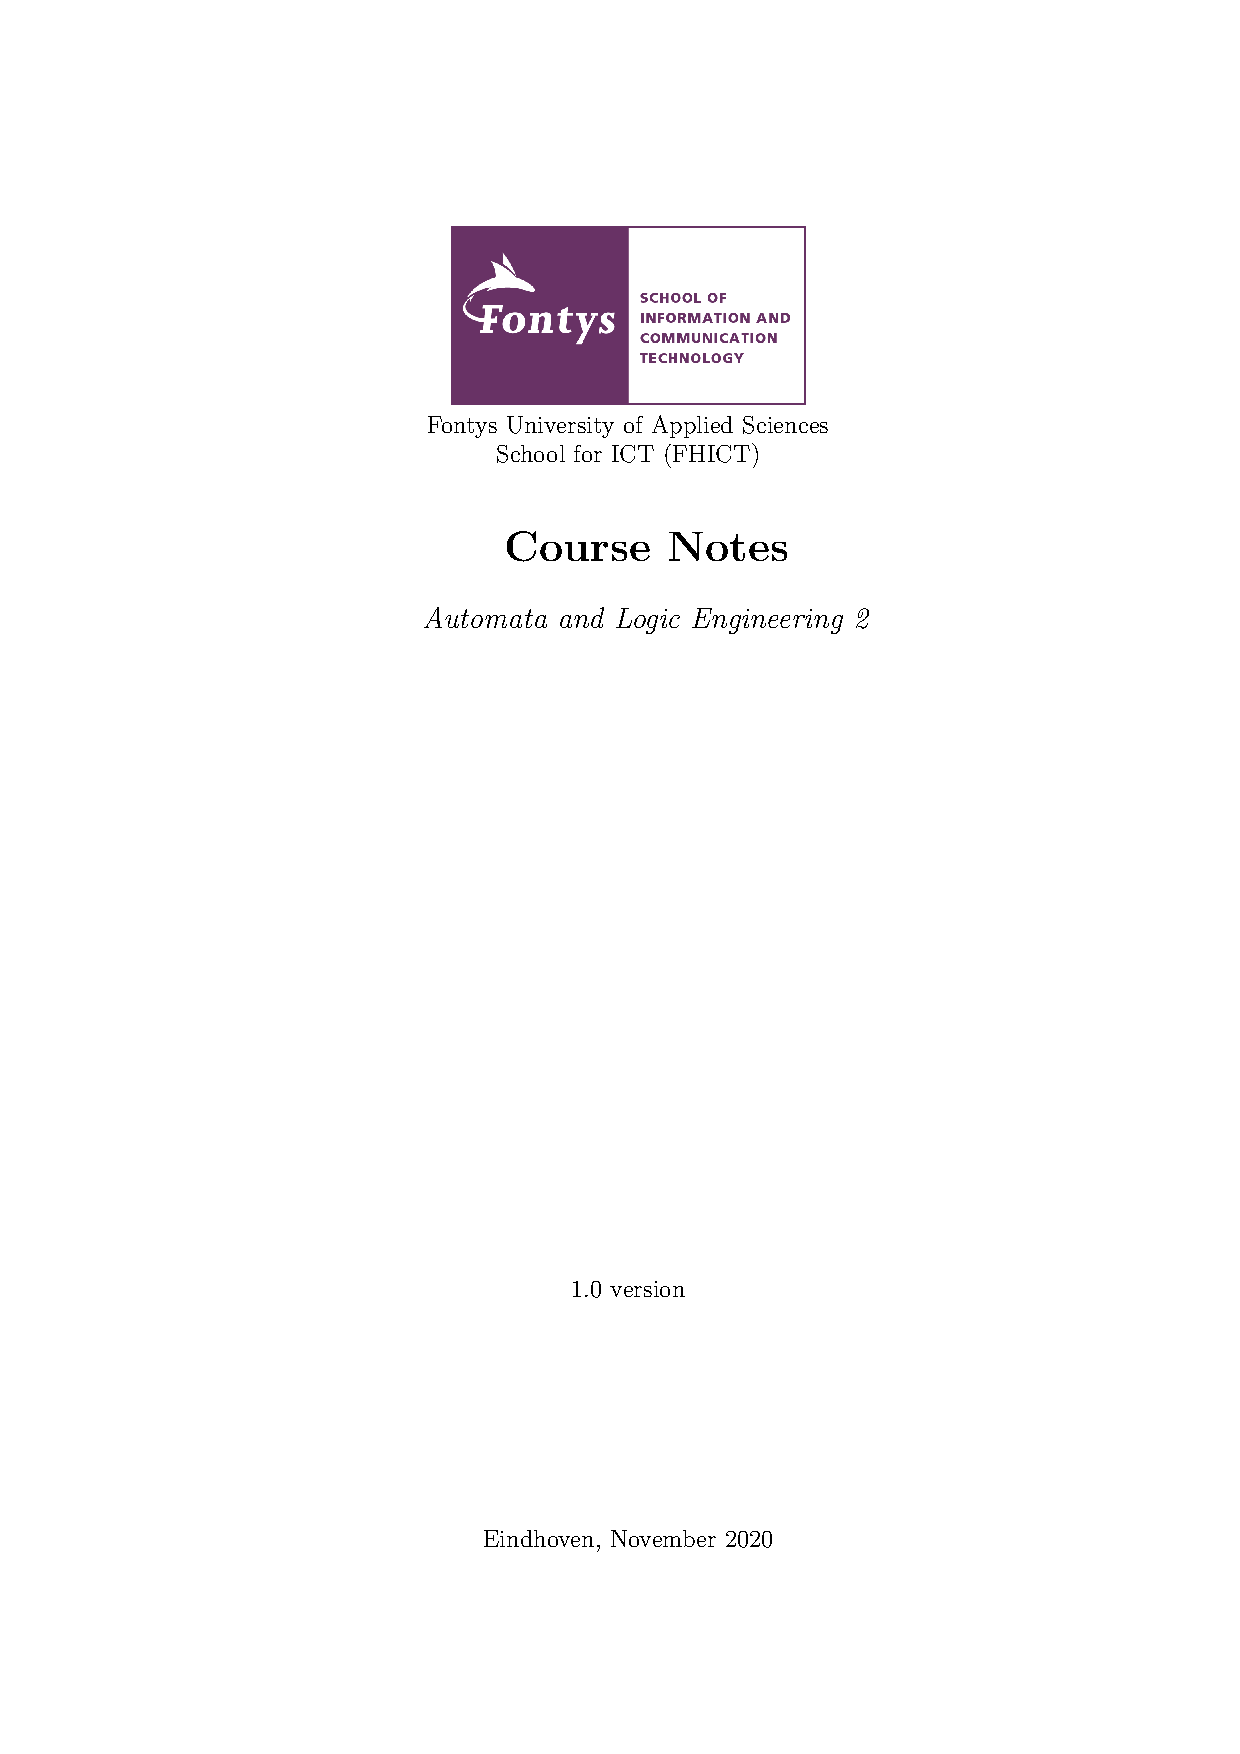
\includepdf[pages=-]{appendices/syllabus/Automata_and_Logic_Engineering_2_Course_Notes}